\documentclass[letterpaper,twoside,notitlepage,12pt]{article}
\usepackage[utf8]{inputenc}
\usepackage[utf8]{inputenc}
\usepackage[margin=1in]{geometry}


\usepackage{csquotes, lipsum, amsmath, amssymb, textcomp, xcolor, verbatim, siunitx, booktabs, multirow, minted}


\usepackage{graphicx}
\graphicspath{ {./} }


\usepackage{hyperref}
\hypersetup{
    colorlinks=true
}


\usepackage{float}
% prevent figure or table from floating to top of page by default
% USAGE: \begin{figure}[H] ...


\usepackage{enumitem}
% control list spacing
% https://tex.stackexchange.com/questions/129951/enumerate-tag-using-the-alphabet-instead-of-numbers
\setlist{noitemsep} 
% also \setlist{nosep} for no space between list & adjacent paragraph

\begin{document}

\noindent
Nikita Zdvijkov \\
EE-1011-01: Comp Tools Elec Engr \\
September 1, 2019

\begin{center}
\large{\textbf{UTulsa ECE Report Template}}
\end{center}

\section{Introduction}

Click \href{https://github.com/nikitazdvijkov/ece-report-template}{here} (\texttt{https://github.com/nikitazdvijkov/ece-report-template}) for more info about this template.

Hint: use the \texttt{\textbackslash input{}} command to organize your code. See what I did for ``table with some cells merged'' section: line 65 of \texttt{main.tex} inserts the content of \texttt{table-with-some-cells-merged.tex} at that point.

\section{Basic examples}

\subsection{Figures}

This is how you reference Figure ~\ref{fig:circuit2}.

\begin{figure}[H]
\begin{center}
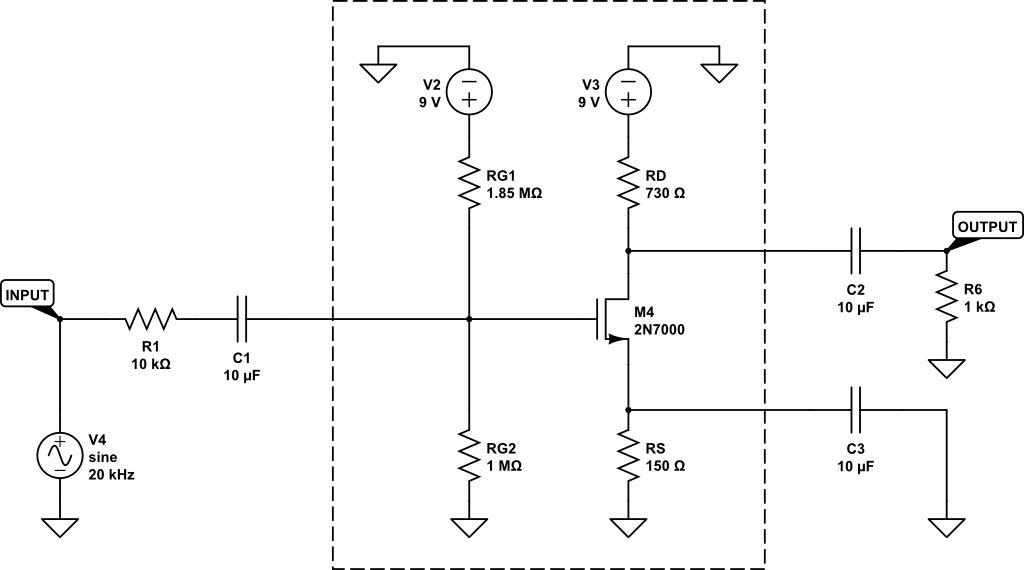
\includegraphics[width=0.9\textwidth]{circuit.png}
\end{center}
\caption{Amplifier circuit}
\label{fig:circuit2}
\end{figure}

\subsection{Simple table}

\begin{table}[H]
\begin{center}
\caption{\small Source-side measured values: $V$, $I$, $P$, $Q$, and $|S|$}
\vspace{5mm}
\begin{tabular}{rrrrr}
\toprule
$V$ ($\text{V}_\text{RMS}$) &
$I$ ($\text{V}_\text{RMS}$) &
$P$ (W) &
$Q$ (VAR) &
$|S|$ (VA) \\ 
\midrule
70.11	& 0.038	& 1.97	& X	& X \\
70.03	& 0.053	& 3.29	& 1.76	& 3.73 \\
70.05	& 0.070	& 4.60	& 1.80	& 4.93 \\
70.01	& 0.088	& 5.89	& 1.80	& 6.15 \\
70.03	& 0.112	& 7.66	& 1.80	& 7.86 \\
69.97	& 0.136	& 9.40	& 1.84	& 9.57 \\
69.96	& 0.161	& 11.11	& 1.84	& 11.25 \\
69.96	& 0.185	& 12.80	& 1.88	& 12.93 \\
69.91	& 0.232	& 16.10	& 1.92	& 16.21 \\
69.88	& 0.278	& 19.35	& 2.00	& 19.45 \\
\bottomrule
\end{tabular}
\end{center}
\end{table}

\subsection{Table with some cells merged}

\begin{table}[H]
\begin{center}

\caption{\small System of equations resolved for the four source pairings}

\vspace{5mm}

\begin{tabular}{ccccccc}

\toprule

\multicolumn{4}{c}{Sources used} 
& \multirow{2}{*}{$\dot{m}_1$ (kg/s)} 
& \multirow{2}{*}{$\dot{m}_2$ (kg/s)} 
& \multirow{2}{*}{$\dot{S}_{\text{gen}}$ (kJ/K)} \\

1 & 2 & 3 & 4 &&& \\

\midrule

X&&X&& 1.671 & 3.329 & 0.1178 \\
X&&&X& 4.603 & 0.397 & 0.4476 \\
&X&X&& 2.782 & 2.218 & 0.0441 \\
&X&&X& 4.833 & 0.167 & 0.1284 \\

\bottomrule

\end{tabular}
\end{center}
\end{table}

\subsection{Code}

\begin{minted}{python}
#!/usr/bin/python3
from html.context import Context

def paragraph(html, line_data):
    line = line_data[0]
    blank_lines = line_data[1] > 1
    if blank_lines:
        html.check_and_close_paragraph()
        html.add('<p>' + line)
        html.push()
        html.need_to_close_paragraph = True
    else:
        html.add(html.expand_line(line))

paragraph_dict = {
    'paragraph':    Context(None, paragraph, None, {})
}
\end{minted}

\end{document}
